\documentclass[a4paper,12pt]{article}
\usepackage[ngerman]{babel}
\usepackage[T1]{fontenc}
\usepackage[utf8]{inputenc}
\usepackage{graphicx}
\usepackage{lmodern}
\usepackage{float}
\usepackage{url}
\usepackage{listings}
\usepackage[nottoc]{tocbibind} %includes the bibtex bibliography into toc
\usepackage{xcolor} %color instead of color for the definecolor >html<
\usepackage{kpfonts}
\usepackage{natbib}

\definecolor{eclipseKeywords}{HTML}{7F0074} %purple %html stands for hexa rgb -> yellow e.g. 255,255,0 = FF FF 00
\definecolor{eclipseComments}{HTML}{3F7F5F} %green
\definecolor{eclipseStrings}{HTML}{2A00FF} %blue
\definecolor{graybackgroundColor}{HTML}{E5E5E5} %gray!20 for gray!30 use D9D9D9 for gray!10 F2F2F2
\definecolor{brownlocalObjects}{HTML}{957D47}

\lstset{
aboveskip=20pt plus2pt minus 4pt,
belowskip=20pt plus2pt minus 4pt,
	numbers=left,
	numbersep=5pt,
	sensitive=false, %groß kleinschriebung
	tabsize=2,
	backgroundcolor=\color{graybackgroundColor},
	showspaces=false,
  showstringspaces=false,
  showtabs=false,
	breaklines=true, %falls der code über den rand herausragt!
		basicstyle=\footnotesize\ttfamily,
	numberstyle=\tiny\ttfamily,
	captionpos=b,
}

\lstdefinestyle{Cpp} {
language=C++,
  keywordstyle=\color{eclipseKeywords},
   stringstyle=\color{eclipseStrings},
  commentstyle=\color{eclipseComments},
  morecomment=[l][\color{eclipseComments}]{\#}
}



\begin{document}

\begin{titlepage}
	\centering
	
\includegraphics[width=0.7\textwidth]{bilder/hskalogo}\par\vspace{1cm}
	\vspace{0.5cm}
	{\Large Studiengang Informatik (Master)}\par
	\vspace{2cm}
	{\huge\bfseries Last-Test von Web-Seiten mit JMeter}\par
	\vspace{2cm}
	{\Large\bfseries Seminararbeit - Ausarbeitung}\par
	\vspace{0.5cm}
	\vspace{3cm}
	
	{\Large Daniel Schäfer (60118)\par}
	\vspace{1cm}
	{\Large\textbf{Betreuer:} Prof.~Dr.~Holger Vogelsang} 
	\vfill
	{\Large Sommersemester 2018\par}
	\vfill
% Bottom of the page
%{\large \today\par}
\end{titlepage}


\tableofcontents
\pagebreak
%\addcontentsline{toc}{section}{Abbildungsverzeichnis}
%\listoffigures

\section{Einführung}
\subsection{Motivation - Wozu überhaupt Testing?}
Man erlebt es immer wieder, dass Webseiten unter zu hoher Last in die Knie gezwungen werden. Sei es nun Amazon, Ebay oder auch Hochschul interne Seiten, die durch bestimmte Anmeldefristen viele Nutzer gleichzeitig versorgen müssen. Doch warum passiert sowas in der heutigen zeit immer noch? Und kann man dem vorbeigeund entgegenwirken? Sogenannte Last oder Performance Test sind dafür nötig. Das frei Verfügbare unter Public License Key stehende Java Programm JMeter bietet diese und weitere funktionalität um die Leistung einer Webseite bis ins kleinste Detail zu analysieren und zu testen.
\subsection{Verschiedene Testarten}
User Acceptance Testing, Compatibility Tests
\subsection{Automatisierte und manuelle Tests}


\section{Apache JMeter}
Auf den ersten Blick erscheint Apache JMeter wie das Relikt aus einer längst vergangenen Zeit. Doch man sollte sich von der Swing-basierten GUI Oberfläche nicht täuschen lassen. 

Tatsächlich stammt JMeter aus einer Zeit als das Web und Application Server noch in den Kinderschuhen steckten.


Man sollte sich jedoch nicht täuschen lassen. Eierlegende  
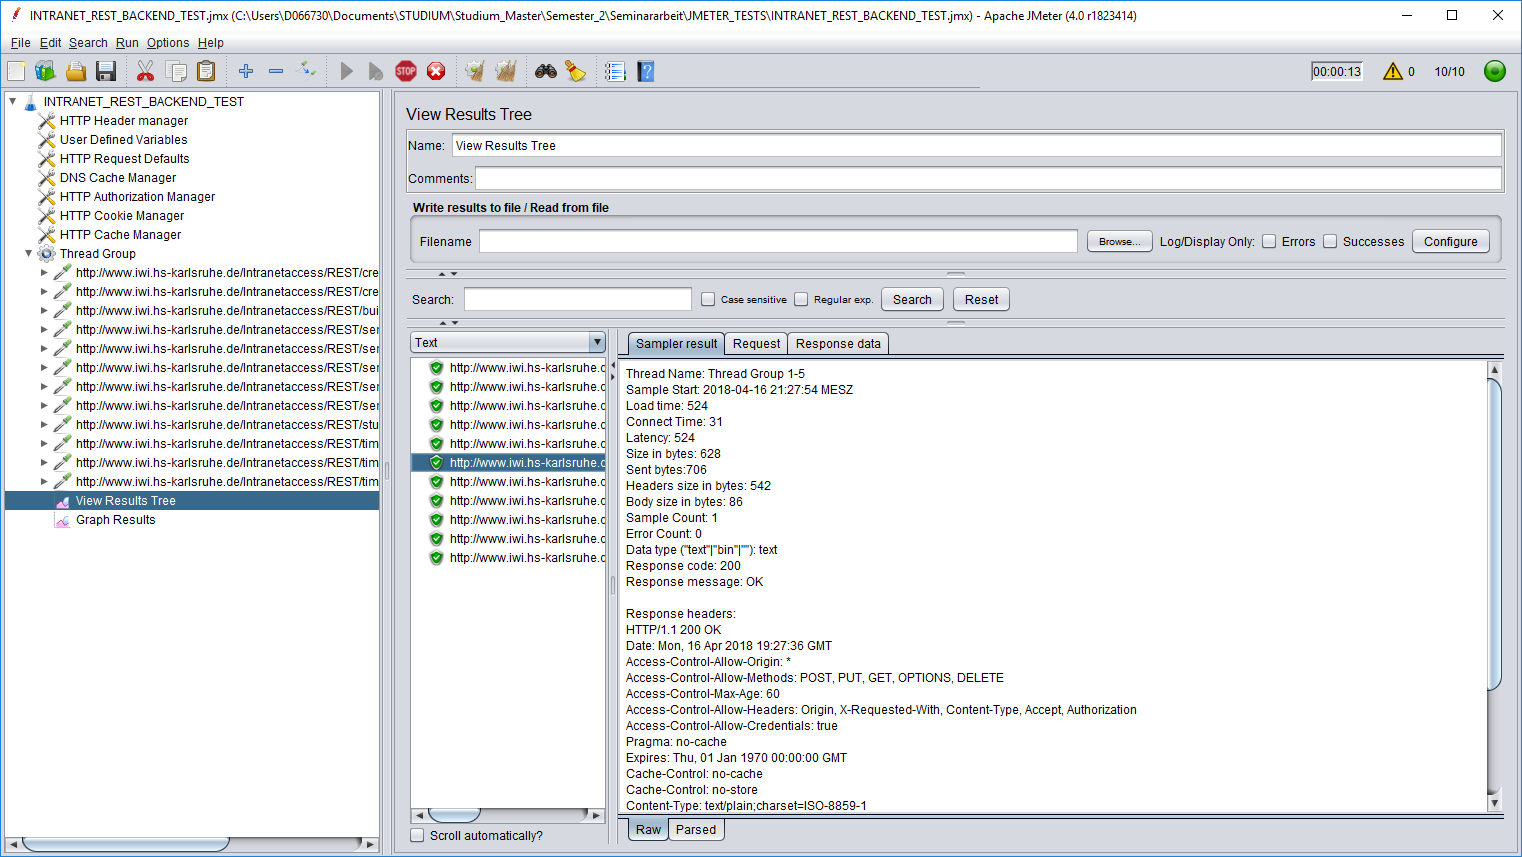
\includegraphics[width=1\textwidth]{bilder/jmeter_1.png}\par\vspace{1cm}
JMeter Platformunabhängig wegen java anwendung. kann sowohl auf mac als auch auf windows laufen. lediglich die java runtime

Wann wurde das Tool das erste mal entwickelt? wie oft wird es eingesetzt. auch von großen unternehmen? kommt bei sap auch zum einsatz

\subsection{Was kann JMeter}

\subsubsection{Lastentests}

\subsubsection{Captcha Analyse}
Captcha analysieren und erkenne?

\subsubsection{Auto vervollständigung von Formularen}
befüllen von formularen

\subsubsection{JUnit Tests}
junit tests in jmeter importieren
\subsection{Installation}
\subsubsection{Setting up the environment}
\subsubsection{Running JMeter}

\subsection{JMeter GUI}
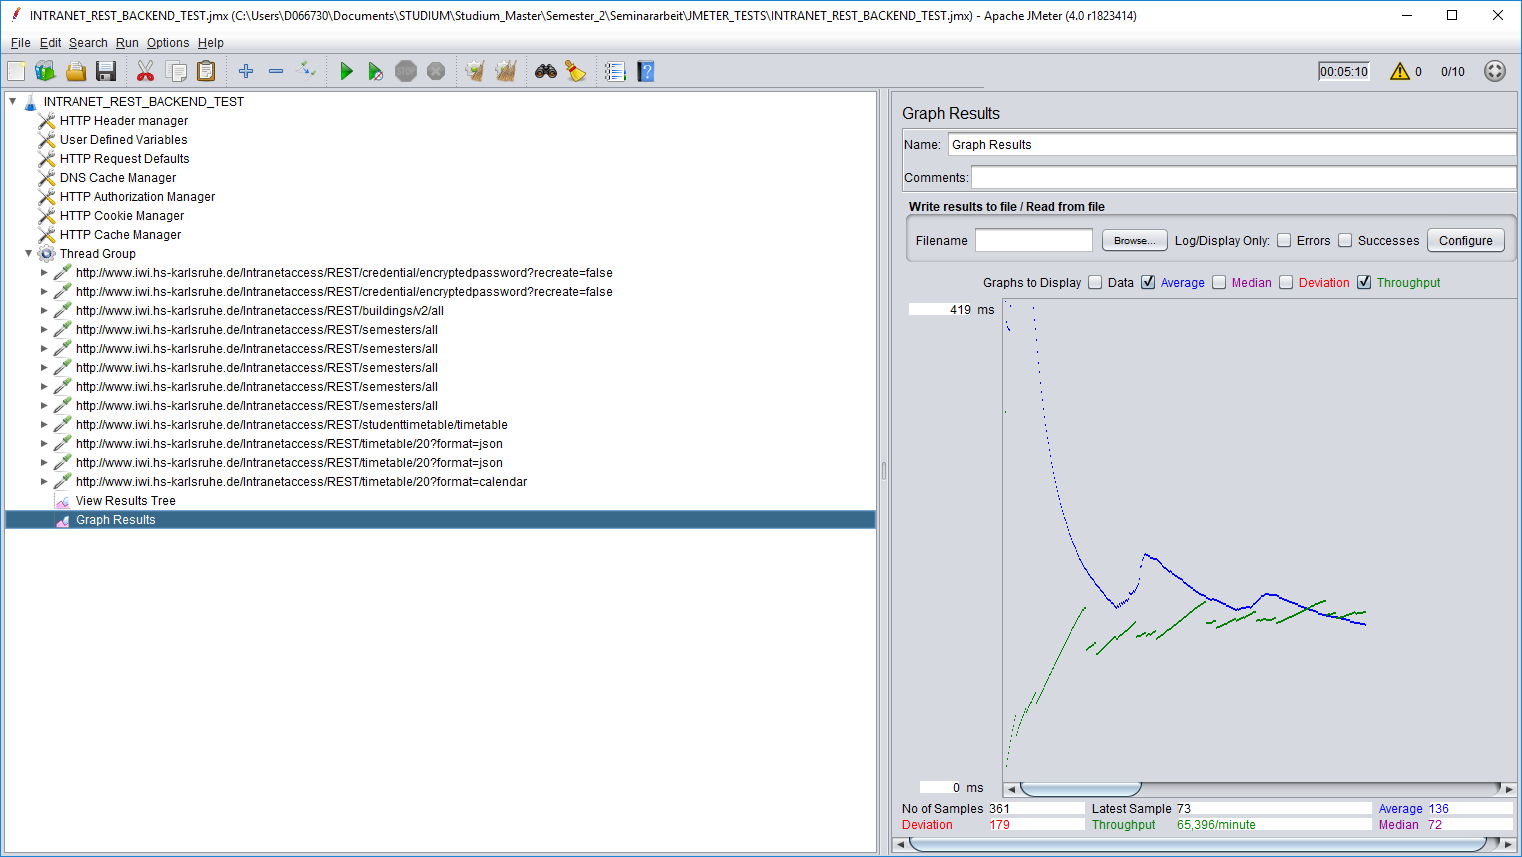
\includegraphics[width=1\textwidth]{bilder/jmeter_2.png}\par\vspace{1cm}

\subsection{JMeter Command Line}
GUI verbraucht viel Speicher. Nicht empfohlen für große Lastentests
Command Line ist geeignet für die Integration in andere Systeme wie Jenkins/Continious Integration
\subsubsection{Ausführen des Console Clients}
Zuerst sollte ein Testscript verfügbar sein. Man kann hier ein vorhandenes File verwenden oder in JMeter selbst ein neues *jmx-File erzeugen. Minimale Voraussetzungen sind eine Thread Group sowie ein Sampler wie etwa ein HTTP Request mit entsprechender URI.

JMeter GUI beenden und Command Line starten. Danch in das /bin Verzeichnis von JMeter navigieren. Dort startet man den Test via dem Befehl:
\begin{lstlisting}[style=Cpp]
  jmeter -n -t [jmx file] -l [results file]
\end{lstlisting}
In der folgenden Tabelle sieht man einige häufig verwendete Parameter und ihre Bedeutung. Um eine Übersicht aller Parameter zu erhalten, kann man in der Console den jmeter -? ausführen.
\begin{table}[H]
	\centering
	\begin{tabular}{|l|l|}
		\hline
		\textbf{Parametername} & \textbf{Bedeutung} \\
		\hline
		-n & non gui mode \\
		-t & location of jmeter script - combined with -n \\
		-l & location of result file \\
		-? & alle Parameter an die zur Auswahl stehen \\
		-h & Beispielbefehle, die man verwenden kann \\
		-L & Log level - Wann soll etwas geloggt werden \\
		-e & Um html Reports zu erzeugen\\
		-o & Location of the output folder - combined with -e or -g \\
		-g & html report wird aus einem csv file erzeugt \\ 
		\hline
	\end{tabular}
	\caption[tab_parameter_non_gui]{Befehle der JMeter Command Line}
	\label{tab_parameter_non_gui}
\end{table}





\section{Der Testplan}
Was ist überhaupt ein Testplan
\subsection{Elemente eines Testplans}
Welche Elemente kann ein Testplan enthalten

1 Testplan anlegen
\subsubsection{Thread-Groups}
Ähnlich wie JUnit. Hier möglichkeiten setup teardown neben den eigentlichen gruppen
Gleichzeitige Benutzer usw.
\subsubsection{Sampler}
Sind die eigentlichen Tests
\subsubsection{Listener}
Elemente die Informationen über die Performance Tests enthalten
Zum abfragen bzw. ergebnisse visualisieren

werden verwendet um ergebnisse und metriken der tests anzuzeigen

\subsubsection{http request}
\subsubsection{Assertions}
Mit jmeter lassen sich assertions testen. Dazu wird der response von einem request untersucht assert 200. assert 500 etc.

\section{Lasttests von Webseiten}

\section{Funktionale Tests}

\section{Wissenswertes und Besonderheiten}
Man kann die Ergebnisse zur Laufzeit in Logfiles schreiben.

\subsection{JMeter Plugin Manager}



\subsection{Aufzeichnen von Aktionen - UI web Test}
Build in Solution:
Bei non-test-Elements Testscript Recorder <-hiermit kann man ein script aufzeichnen um ganze Webseiten zu untersuchen

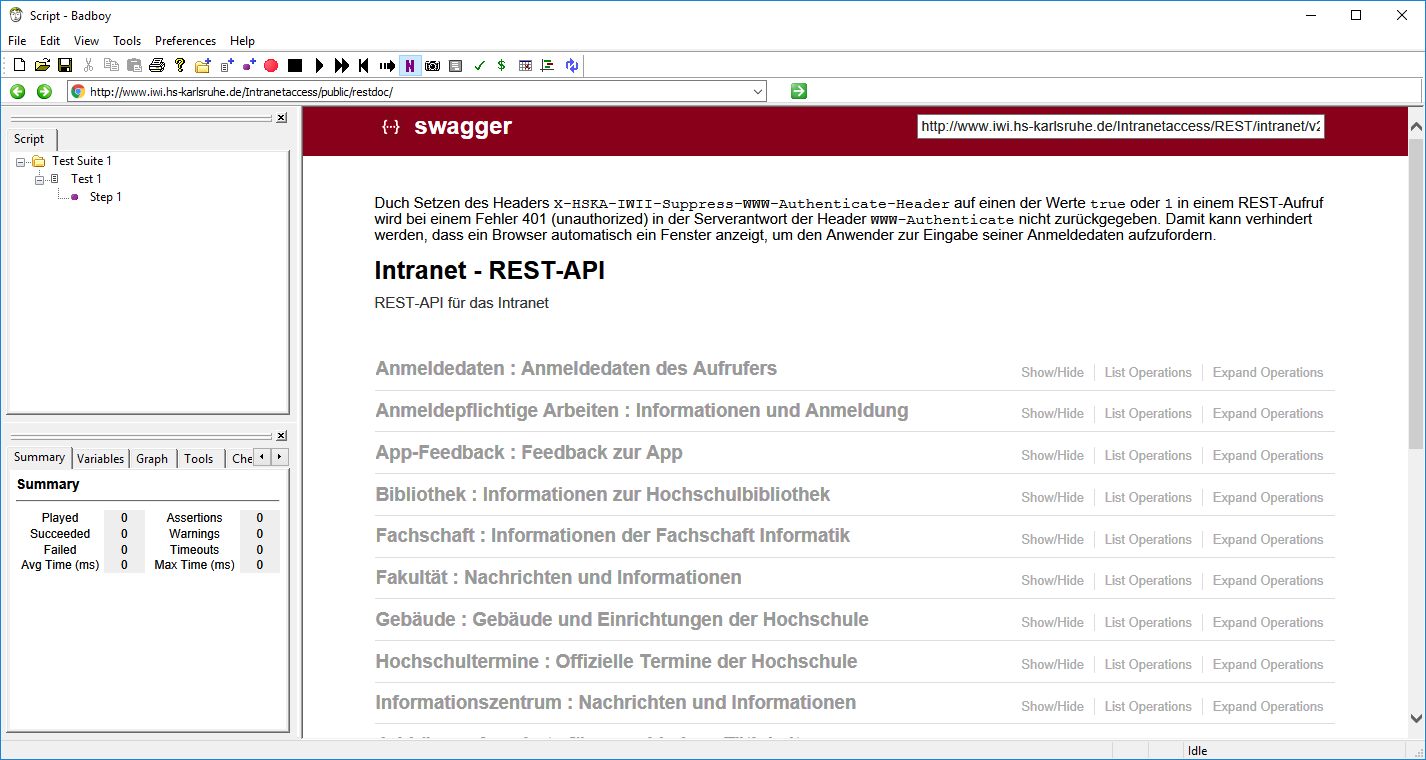
\includegraphics[width=1\textwidth]{bilder/badboy.png}\par\vspace{1cm}
Für Windows only Platformabhängig BadBoy:
Ansonsten drittanbieter verwenden wie etwa badboy.

Chrome Plugin:
Blazemeter
Mit Blazemeter ist man in der Lage direkt in Chrome und somit platformunabhängig Aufzeichnungen von Aktionen auf Webseiten aufzunehmen.
Kleiner Nachteil: Man muss sich bei Blazemeter registrieren um den Export in .jmx Dateien ausführen zu können.
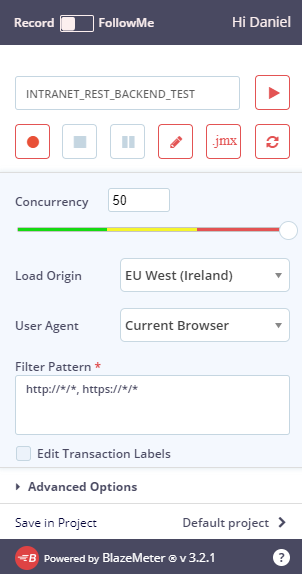
\includegraphics[width=0.5\textwidth]{bilder/blazemeter.png}\par\vspace{1cm}

\subsection{Datenbankabfragen - Datenbank testplan?}
Auch datenbankabfragen lassen sich damit visualisieren

Falls interersse besteht, wie es funktioniert bitte in die Ausarbeitung schauen.
Thread Gruppe erstellen -> Configuration (JDBC Connection Configuration)
MySQL jdbc jar in lib folder von jmeter adden 
DAnn Sampler -> JDBC Request and put in values.. z.b. select * from table


\subsection{Virtuelle Compute Unit}
In die Cloud um an einer zentralen stelle viele rechner zu bedienen?
Eventuell viele Rechner simulierenö

\subsection{JMeter change Settings}
In /bin folder von JMeter kann man die Datei user.properties öffnen und Werte anpassen.

\section{Nachteile von JMeter}
Wenn ein Variablenfeld required ist. z.b. bei JDBC Connection Configuration. dann wird einem der fehler nicht direkt im feld angezeigt.

Ziemlich resourcenhungrig. Trotz 16GB Arbeitsspeicher hängt sich das Ding gerne mal auf.
\section{Fazit}
Alles in allem ist JMeter ein Super tool

\pagebreak
\bibliographystyle{plain}
\bibliography{bibliography}

\end{document}